\chapter{Method}
\label{chap:method}
For our experiments, we follow the steps depicted in Figure \ref{fig:pipeline}.
\begin{figure}[ht]
    \centering
    
\includegraphics[width=1.0\linewidth]{img/pipeline.png}
    % \includesvg[pretex=\tiny, width=1.0\linewidth]{img/pipeline}
    \caption[Visualization of the pipeline the thesis built upon]{Visualization of our pipeline for \ac{lod} generation. Yellow boxes represent files that are inputs our outputs of green program components. Evaluation is partially done by visual comparison and by computing image quality metrics.}
    \label{fig:pipeline}
\end{figure}
We first take the surface meshes and apply the filtering procedure to obtain the volume grids.
Additionally we save metadata like the bounding-box sizes of the grids, which we then need for scene generation.
This generation step can either generate ground-truth scenes that only contain meshes or it can generate scenes that use \acp{lod}.
The next step in the pipeline is the rendering of the scene, which uses mesh or volume files depending on the definitions in the generated scene file.
Finally we evaluate our results by comparing the mesh-only renderings with the ones that use \ac{lod}.
This is done regarding the image quality and the render performance between the mesh-only renderings and the \ac{lod} renderings.
We are however not interested in the absolute render times, but rather in the relative times between the mesh and volume representations.
This final evaluation step is explained in Chapter \ref{chap:results_and_discussion} while all other steps are subject of this chapter.

Although our pipeline can be used with arbitrary models, we only use tree models with it.
In total these are 26 free tree meshes from XfrogPlants \cite{xfrogplants} and the McGuire Computer Graphics Archive \cite{McGuire2017Data} which are available as \texttt{.obj} files with the textures being encoded as \texttt{.png} or \texttt{.tiff}.
Meshes and textures together occupy 1.2 GB of disk memory.
Apart from the models itself, XfrogPlants also provides information of the sizes the trees grow during their lifespan, which we also need during filtering and scene generation.

\section{Mesh filtering}
\label{sec:mesh_filtering}
As described in Section \ref{sec:transforming_meshes_into_volumes} we use the ray casting approach by \citeauthor{hybrid_mesh_volume_lods} with a few modifications for our filtering \cite{hybrid_mesh_volume_lods}.
The ray casting is \ac{gpu} accelerated using OptiX \cite{parker_optix}.
In contrast to \citeauthor{hybrid_mesh_volume_lods} we assume our particles to have an isotropic microflake projected area $\sigma$, meaning that it is not view dependent.
This greatly simplifies our optimization procedure as well as the distance sampling and transmittance estimation later during rendering.

During filtering we place the voxel grid over the mesh and align it to three sides of the bounding box of the mesh.
If the edge lengths of the mesh's bounding box do not evenly divide by the size of a voxel, we let the volume overlap on the non-aligned sides.
In each voxel we then sample the origin of our rays on a cubic uniform domain and the direction of the rays is uniformly sampled over the unit sphere.
\citeauthor{hybrid_mesh_volume_lods} use a ray length that is equal to the edge length of a voxel, which leads to a blurring since adjacent geometry is included in the density estimation.
As \citeauthor{wang_object_space_aliasing} points out, this can reduce object space aliasing \cite{wang_object_space_aliasing}.
However we think, that we can increase the spatial resolution while preserving the blurring by clipping the ray at a bounding sphere.
We position the sphere at the voxel's center and scale it so that its diameter is slightly larger than the diagonal of the voxel.
Each ray is then first intersected with this sphere to compute a $t_{max}$, before the intersection test with the mesh geometry happens.
Figure \ref{fig:raygen_filtering} compares our approach for determining the ray length with the approach of \citeauthor{hybrid_mesh_volume_lods}.
\begin{figure}[ht]
    \centering
    \begin{subfigure}[b]{0.25\linewidth}
        \centering
        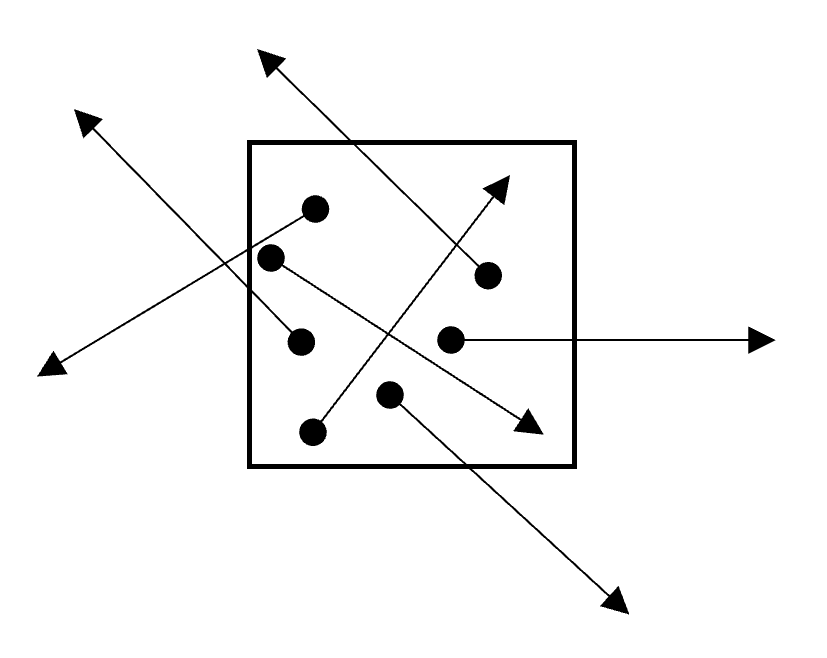
\includegraphics[width=\linewidth]{img/raygen_filtering_unclipped.png}
        \caption{}
        \label{fig:raygen_filtering_unclipped}
    \end{subfigure}
    \begin{subfigure}[b]{0.25\linewidth}
        \centering
        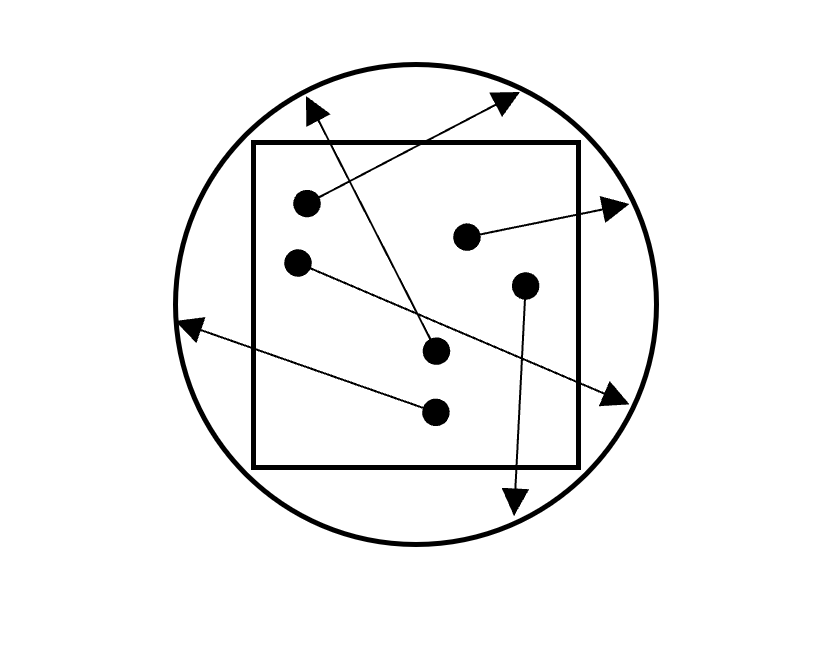
\includegraphics[width=1\linewidth]{img/raygen_filtering_clipped.png}
        \caption{}
        \label{fig:raygen_filtering_clipped}
    \end{subfigure}
	\caption[Approaches for determining a ray length for filtering]{Image (a) shows the approach by \citeauthor{hybrid_mesh_volume_lods} with constant ray length. Figure (b) shows our approach with ray clipping at a bounding sphere.}
	\label{fig:raygen_filtering}
\end{figure}

With these modifications we also have to solve a different integral than that from Equation \ref{eq:loubet_filtering_equation}.
We therefore have to find a density $\rho$ that suffices:
\begin{equation}
    1 - \frac{1}{4\pi}\int_{\mathcal{S}^2} e^{-\rho\sigma ray_l(\omega)} d\omega = P_{occ}.
    \label{eq:our_filtering_equation}
\end{equation}
Note that the projected area $\sigma$ is now independent of the direction $\omega$, whereas the ray length depends on $\omega$, since the rays are clipped by the bounding sphere.
As stated in Section \ref{sec:transforming_meshes_into_volumes}, we cannot solve for the density with analytical methods, therefore we iteratively optimize $rho$:
\begin{equation*}
    \rho_{i+1}=\rho_i - \alpha (P_{occ,volume} - P_{occ,mesh}),
\end{equation*}
where $i$ denotes the iteration, $\alpha$ is a learning rate, $P_{occ,mesh}$ is the ratio of geometry hits to the total number of rays casted and $P_{occ,volume}$ is the probability that a medium interaction takes place given the density $\rho$.
It is computed by Monte Carlo integrating Equation \ref{eq:our_filtering_equation}, so our estimator has the form:
\begin{equation*}
    1 - \frac{1}{N}\sum_{n=1}^{N} e^{-\rho\sigma ray_l(\omega_n)} = P_{occ,volume}.
\end{equation*}
Apart from this density estimate we also filter the diffuse and specular color of the geometry, the normals, the index of refraction and the SGGX Matrix $S$ by averaging.
The Matrix $S$ serves later as a coordinate frame for sampling reflection directions with the phase function \cite{sggx}.

% In total our attributes occupy 80 bytes of memory per voxel and we first represent them by a dense grid in the \ac{GPU}'s global memory.
We represent these attributes as a dense grid in the \acs{gpu}'s global memory.
OpenVDB cannot be used for this, because it is incompatible with CUDA device code \cite{museth_nanovdb}, NanoVDB on the other hand, is a read-only grid \cite{nanovdb}.
Only after copying the dense grid to host memory we convert it into an OpenVDB grid and subsequently into a NanoVDB grid which we store to disk.
Using NanoVDB however, imposes a limit of storing 32 bytes per voxel which we can't increase in the limited time frame of the thesis \cite{open_to_nanovdb}.
Because our attributes occupy 80 bytes of memory, we use quantization to represent the values in the grid and before doing computations like interpolation or shading, we transform them back to the full width.
The following table summarizes the size of all attributes in regular and quantized format (ignoring padding):
\begin{center}
    \begin{tabular}{| c | c | c | }
        \hline
         & Regular Format & Quantized Format \\
         \hline
         Density & $1\times 4\;\text{bytes}$ & $1\times 4\;\text{bytes}$ \\
         \hline
         $S$ & $9\times 4\;\text{bytes}$ & $6\times 2\;\text{bytes}$ \\
         \hline
         Diffuse color & $3\times 4\;\text{bytes}$ & $3\times 1\;\text{bytes}$ \\
         \hline
         Specular color & $3\times 4\;\text{bytes}$ & $3\times 1\;\text{bytes}$ \\
         \hline
         Normal & $3\times 4\;\text{bytes}$ & $3\times 2\;\text{bytes}$ \\
         \hline
         Index of refraction & $1\times 4\;\text{bytes}$ & $1\times 2\;\text{bytes}$ \\
         \thickhline
         Total & $80\;\text{bytes}$ & $30\;\text{bytes}$ \\
         \hline
    \end{tabular}
\end{center}
Note that since $S$ is a symmetric matrix, it is enough to store six coefficients \cite{sggx}.
Apart from storing the NanoVDB grid we also store the brick grid, which only contains the density values of each voxel.
In principle, it would be possible to store all voxel attributes in brick grid, though the performance gain would be small and modifying brick grid to support this would take some time.
For every \ac{lod} we also export metadata which encompasses the number of voxels in the grid and the bounding box dimensions during filtering.

We generate 7 \acsp{lod} for voxel sizes from 0.1m to 6.4m, doubling the size of a voxel for each \ac{lod}.
The number of voxels is then computed from the voxel size and the size of the trees.
The reason for choosing a voxel size between 0.1m and 6.4m is because for finer voxels the grids quickly use more memory than their surface representations while choosing even larger sizes has no effect, since some trees are already represented by a single voxel on the coarsest level.
The resulting grids occupy 940MB of disk space, where the finest \acsp{lod} are responsible for 65\% of this data.
In chapter \ref{chap:results_and_discussion} we discuss how dropping this \ac{lod} affects image quality and rendering times.

Having the \acsp{lod}, Figure \ref{fig:lods_comparison} compares them to the surface representation for some models.
\begin{figure}[ht]
    \begin{center}
        \begin{tabularx}{\textwidth}{ X  X  X  X  }
            \hline
            Model & Mesh & Volume \newline(Voxel size = 0.1m) & Volume \newline(Voxel size = 0.8m) \\
            \hline
            Acer\newline rubrum\newline adult & \adjustimage{height=3.9cm,valign=m}{img/EA01a_mesh.png} & \adjustimage{height=3.9cm,valign=m}{img/EA01a_0.1.png} & \adjustimage{height=3.9cm,valign=m}{img/EA01a_0.8.png} \\
            \hline
            Acacia\newline sophorae 9 & \adjustimage{height=3.9cm,valign=m}{img/OC41_9_mesh.png} & \adjustimage{height=3.9cm,valign=m}{img/OC41_9_0.1.png} & \adjustimage{height=3.9cm,valign=m}{img/OC41_9_0.8.png} \\
            \hline
            Celtis\newline australis\newline medium & \adjustimage{height=3.9cm,valign=m}{img/EU06m_mesh.png} & \adjustimage{height=3.9cm,valign=m}{img/EU06m_0.1.png} & \adjustimage{height=3.9cm,valign=m}{img/EU06m_0.8.png} \\
            \hline
            Pinus\newline muricata\newline adult & \adjustimage{height=3.9cm,valign=m}{img/CL13a_mesh.png} & \adjustimage{height=3.9cm,valign=m}{img/CL13a_0.1.png} & \adjustimage{height=3.9cm,valign=m}{img/CL13a_0.8.png} \\
            \hline
        \end{tabularx}
    \end{center}
    \caption[Comparison between mesh and volume renderings]{Comparison between the surface representation in the first column and two different \acsp{lod} in columns two and three.}
    \label{fig:lods_comparison}
\end{figure}

\section{Scene Generation}
\label{sec:scene_generation}
We implement the scene generator in Python.
It uses the volume metadata that is exported during filtering and generates a circular forest with uniformly distributed trees.
Our generator uses a rejection sampling approach, rejecting samples that are too close to another.
It is therefore similar to a poisson disk sampler \cite{poisson_sampling}, however it uses varying spacing between the samples depending on the model size.
This is why we exported the bounding box sizes of the volumes during filtering.
First we identify the largest bounding box for each model.
Differences in the bounding box size of a model can occur, because during filtering we make sure that the mesh is fully enclosed by voxels for a given voxel size.
This effect is visualized in Figure \ref{fig:bounding_sizes}.
\begin{figure}[ht]
    \centering
    \begin{subfigure}[b]{0.45\linewidth}
        \centering
        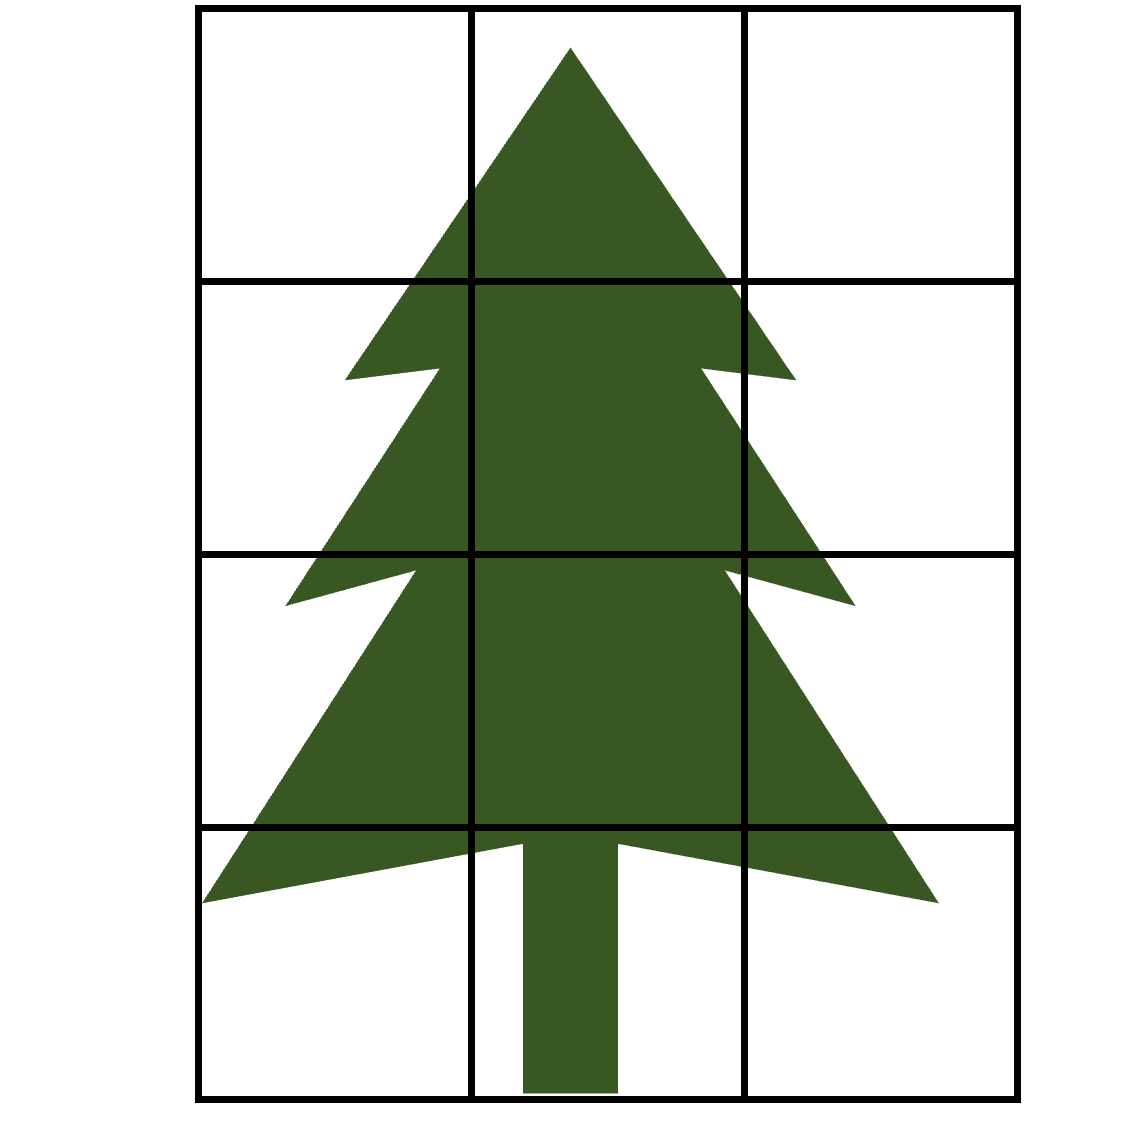
\includegraphics[height=4cm]{img/bounding_size_1.png}
        % \caption{}
        % \label{fig:bounding_size_1}
    \end{subfigure}
    \begin{subfigure}[b]{0.45\linewidth}
        \centering
        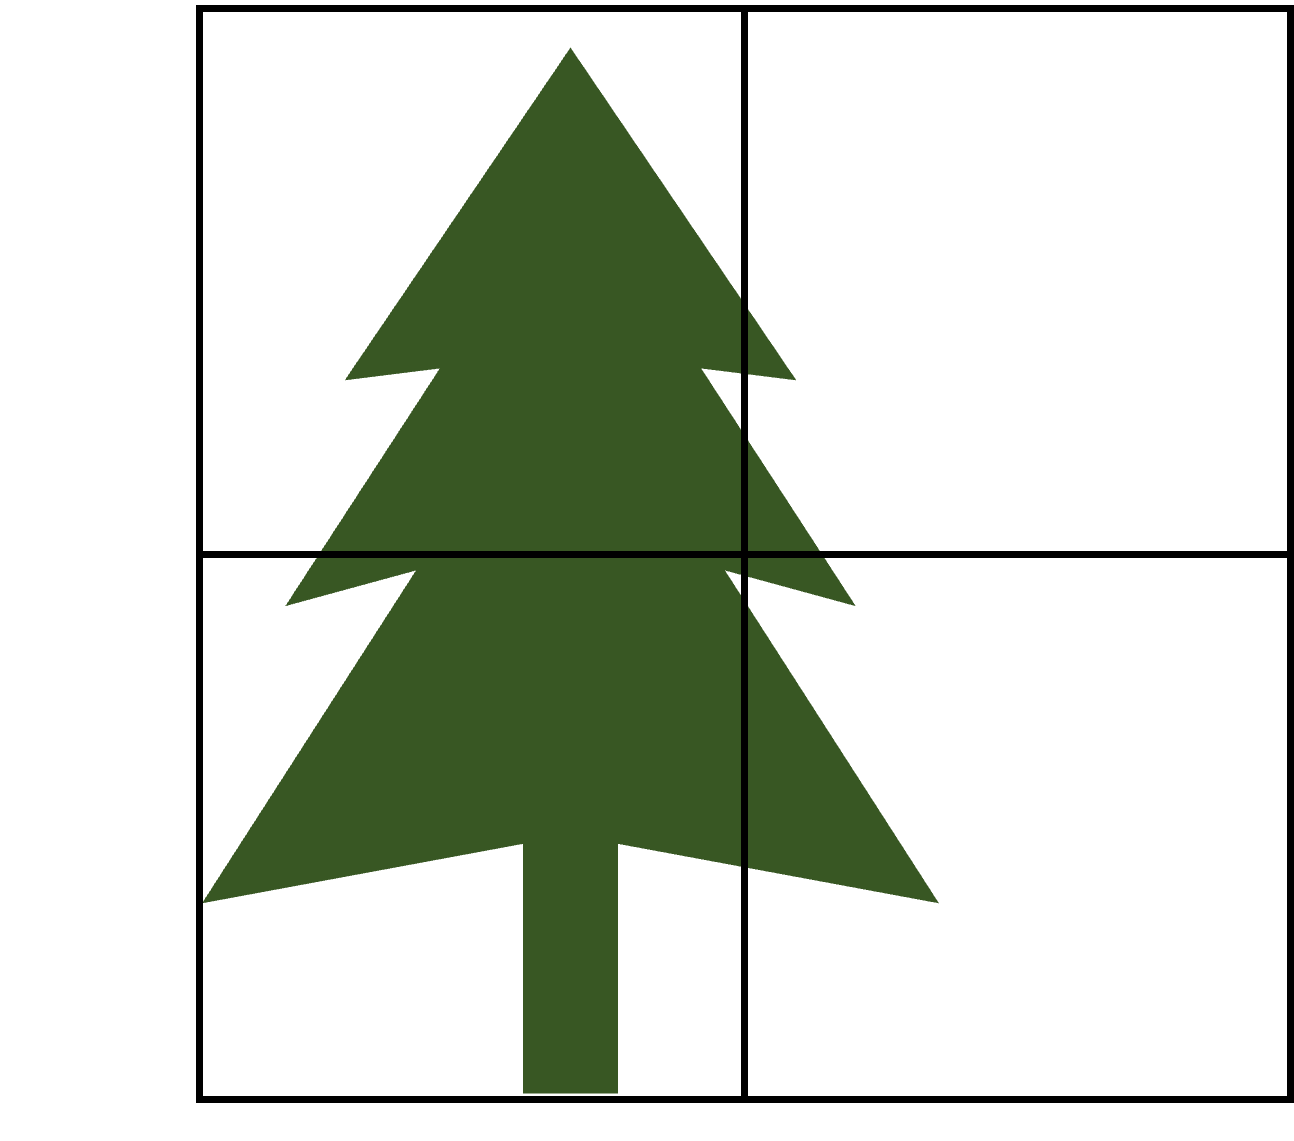
\includegraphics[height=4cm]{img/bounding_size_2.png}
        % \caption{}
        % \label{fig:bounding_size_2}
    \end{subfigure}
	\caption[Bounding boxes resulting from different sized voxels]{The volume is always aligned to one side of the mesh. If we have different sized voxels (like \acsp{lod} necessarily have) the volume overlaps on one side and the bounding box sizes differ.}
	\label{fig:bounding_sizes}
\end{figure}
Then we sample a class \textit{Large}, \textit{Medium}, \textit{Small}, which contain tree models in the corresponding sizes.
We assign trees that grow 20-35 meters to the class \textit{Large}, trees that reach 10-20 meters are labeled as \textit{Medium} and trees that are smaller than 10 meters are assigned to the \textit{Small} class.
This allows us to control the age of the forest.
For example, if we want an old forest we increase the probability for class \textit{Large} and if we want a rather young forest we increase the probability for \textit{Small} trees.
We then choose a tree from this class, sample a position in the circle and check whether it collides with existing models.
This step is a significant performance bottleneck for all rejection based sampling procedures.
In our case we need 100000 sample positions to generate a scene with only 9924 trees.
For all of these sampled positions we have to test whether the models overlap.
In order to accelerate this we employ a spatial acceleration structure: Since our forest has circular shape, we subdivide this circle into concentric segments.
We then have to check for a collision only in the segments in which our model is located.
The collision test itself is based on cylinders around the bounding boxes of the models, which may not overlap.
This acceleration reduces the scene generation with our Python script to a managable runtime of 6 minutes.

Having successively sampled an empty place in the circular forest we still get an overlap if we place a model at this exact position.
The reason is that the bounding box of the model might be asymmetrical.
For example: Consider a bounding box $BB_{min}=(-2.5, -5.0)$, $BB_{max}=(6.0, 10.0)$ and a sampled location $Pos_{center}=(1.5, 3.0)$.
The sampled location gives us the position where the \textit{center} of the bounding box namely $BB_{center}=(1.75, 2.5)$ has to be located.
However, all transformation matrices we use operate on the \textit{origin} of the model space.
Thus we have to compute the position of the origin in world space using:
\begin{equation*}
    Pos_{origin}=\frac{2Pos_{center}-Scale(BB_{min}+BB_{max})}{2},
\end{equation*}
where $Scale$ is an additional scaling factor for controlling the size of the model.
In our example, assuming a scaling of 1, this gives a location for the model of $Pos_{origin}=(-0.25, 0.5)$.

If we generate a ground truth scene, meaning that it contains only mesh models, we can now add the model to the scene, else we now have to determine the appropriate \ac{lod} for the model given the distance to the camera.
Knowledge of the camera position, gaze direction, the \ac{fov} and the sensor resolution are essential for that.
Note that a consequence is, that this information is baked into the scene description and moving the camera during rendering leads to a mismatch of the \acp{lod}.
Generating the scene in the renderer on the fly is currently no option, since this would lead to significantly worse performance of the renderer.
For positions outside the view frustum, we choose the coarsest \ac{lod} since these are not visible and only participate in indirect lighting.
If the position is inside the view frustum, we project the eight bounding box vertices of the coarsest volume on the image plane and compute the area of their convex hull using \texttt{scipy.spatial.ConvexHull} \cite{scipy}.
This gives us the number of pixels that the volume covers on the sensor.
We want to select \acp{lod} based on the heuristic that each voxel covers at most one pixel:
\begin{equation*}
    \frac{n_{voxel}}{n_{pixel}} > 1.
\end{equation*}
Therefore, we now have to compute the number of voxels that we see.
Calculating the product of the number of voxels in depth, height and width gives too many voxels, since some of the voxels are hidden by others.
Computing $depth \times height$, $depth \times width$ or $height \times width$ is only valid for viewing angles that are perpendicular to the surface of the voxel grid.
Another approach is to position a plane at the center of the grid and orient it towards the camera.
The number of voxels that this plane intersects would then be a ground truth value for the voxels that we see.
Evaluating this however, is really expensive since each voxel has to be tested whether it intersects the plane.
We choose a faster approach that approximates this value and is depicted in Figure \ref{fig:voxel_estimation}.
\begin{figure}[ht]
    \centering
    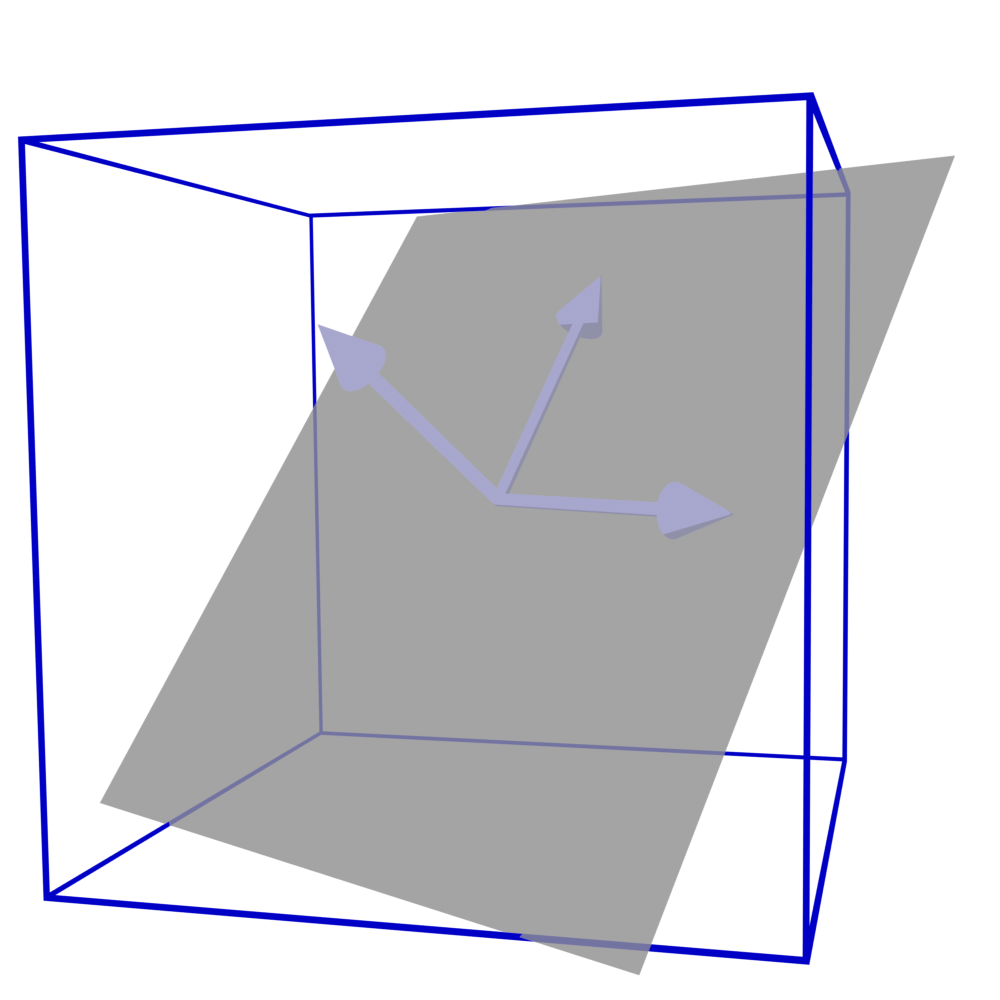
\includegraphics[width=0.3\linewidth]{img/voxel_estimation.png}
    % \includesvg[pretex=\tiny, width=1.0\linewidth]{img/pipeline}
    \caption[Estimation of intersected voxels]{We estimate the number of intersected voxels by shooting two rays which are perpendicular to the camera direction (plane normal). After intersecting them with the bounding box we can construct a rectangle whose area approximates the number of voxels intersected by a plane. The true value is different, since a plane intersecting a cube can produce anything from a triangular to a hexagonal area.}
    \label{fig:voxel_estimation}
\end{figure}
From the center of the volume bounding box we shoot a ray perpendicular to the camera direction horizontally.
A second ray is shot in a direction perpendicular to the first ray and perpendicular to the direction towards the camera.
We intersect the rays with the bounding box which gives us the number of voxels they passed.
By multiplying the results from both rays we get the number of voxels a rectangle located at the bounding box center intersects.
The ground truth value for the number of intersected voxels by a plane can be different, since a plane intersecting a cube does not necessarily give a rectangle.
However we found that our approach closely approximates the true value.
Having computed the number of voxels we can now choose the coarsest \ac{lod} that still fulfills our heuristic and add it to our scene.

As written before we repeat this procedure 100000 times to get a scene with 9924 trees, which are distributed over a circular area with a radius of 1000 meters.
Figure \ref{fig:visualize_lods} shows this scene rendered from the top with colored bounding boxes of the volumes.
\begin{figure}[ht]
    \centering
    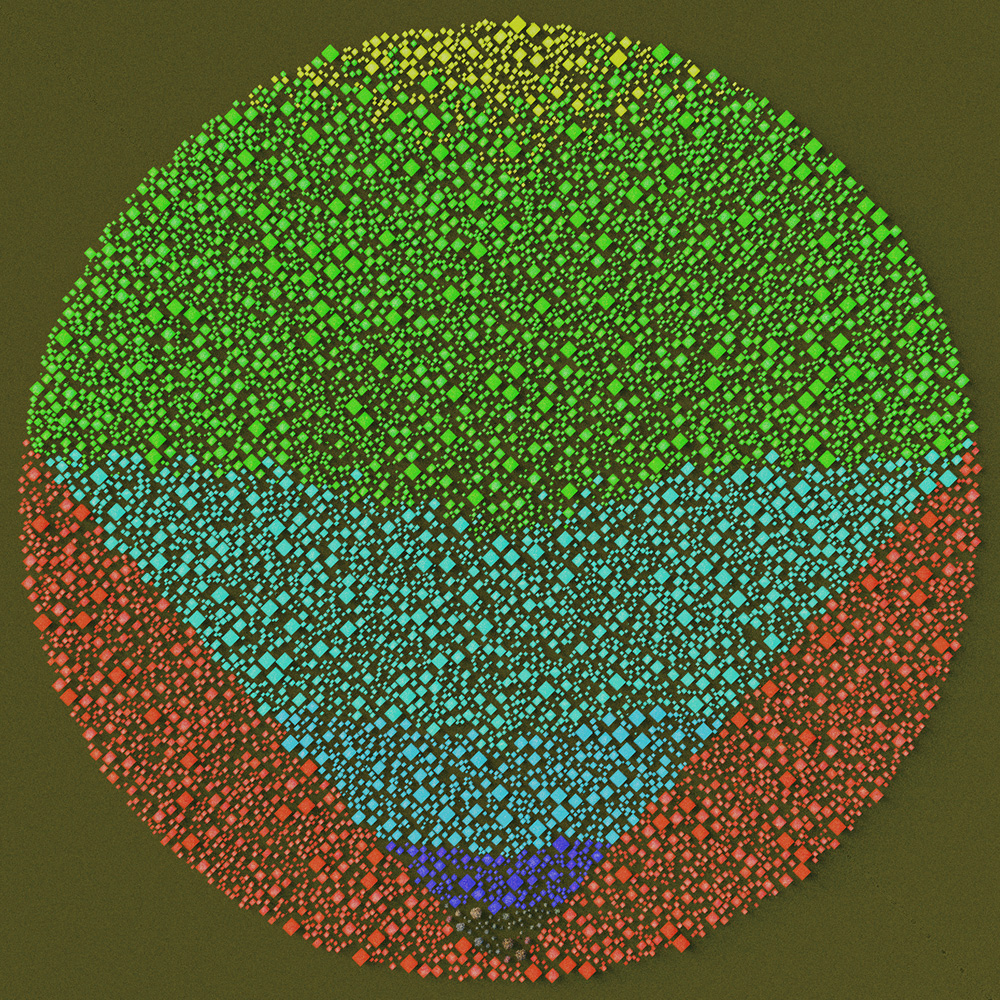
\includegraphics[width=0.5\linewidth]{img/visualize_lods.jpg}
    % \includesvg[pretex=\tiny, width=1.0\linewidth]{img/pipeline}
    \caption[Visualization of a \ac{lod} scene]{Visualization of a debug view of the generated scene using our heuristic. The different voxel sizes between each \ac{lod} are visualized by different colors of the bounding boxes. The colors range from blue, which represents the finest \ac{lod} with a voxel size of $\SI{0.1}{m}$, to red which represents the \acsp{lod} with a voxel size of $\SI{6.4}{m}$.}
    \label{fig:visualize_lods}
\end{figure}
It is clearly visible that we start rendering with meshes and then switch to successively coarser \acsp{lod} with further distance from the camera.
Additionally we see the frustum of the camera: Within the view frustum we select between different \acsp{lod} while we simply choose the coarsest \ac{lod} with a voxel size of 6.4 meters outside the frustum.


\section{Rendering}
\label{sec:rendering}
We render meshes and volumes using path tracing.
Like our filtering implementation, our path-tracer is also \ac{gpu} accelerated using OptiX \cite{parker_optix}.
For fast convergence we employ next event estimation and use importance sampling of the scattering functions and the environment map.
Russian roulette is used to terminate insignificant paths.
In order to render scenes with many meshes and volumes, we use instancing.
A certain mesh or volume thus has to occupy \ac{gpu} memory just once and for each usage an instance is created, each with its own model transformation.
We do the same for textures, loading only textures that differ in their file path.
Each material then stores a pointer to the memory location of the texture.

Our surfaces use the lambertian diffuse \cite{lambert} and the Trowbridge-Reitz microfacet \ac{brdf} \cite{trowbridge_reitz}, which is the general form of the GGX \ac{brdf}.
As Figure \ref{fig:leaf_gloss} shows, real leafs can have a specular gloss, therefore we incorporate a specular \ac{brdf}.
\begin{figure}[ht]
    \centering
    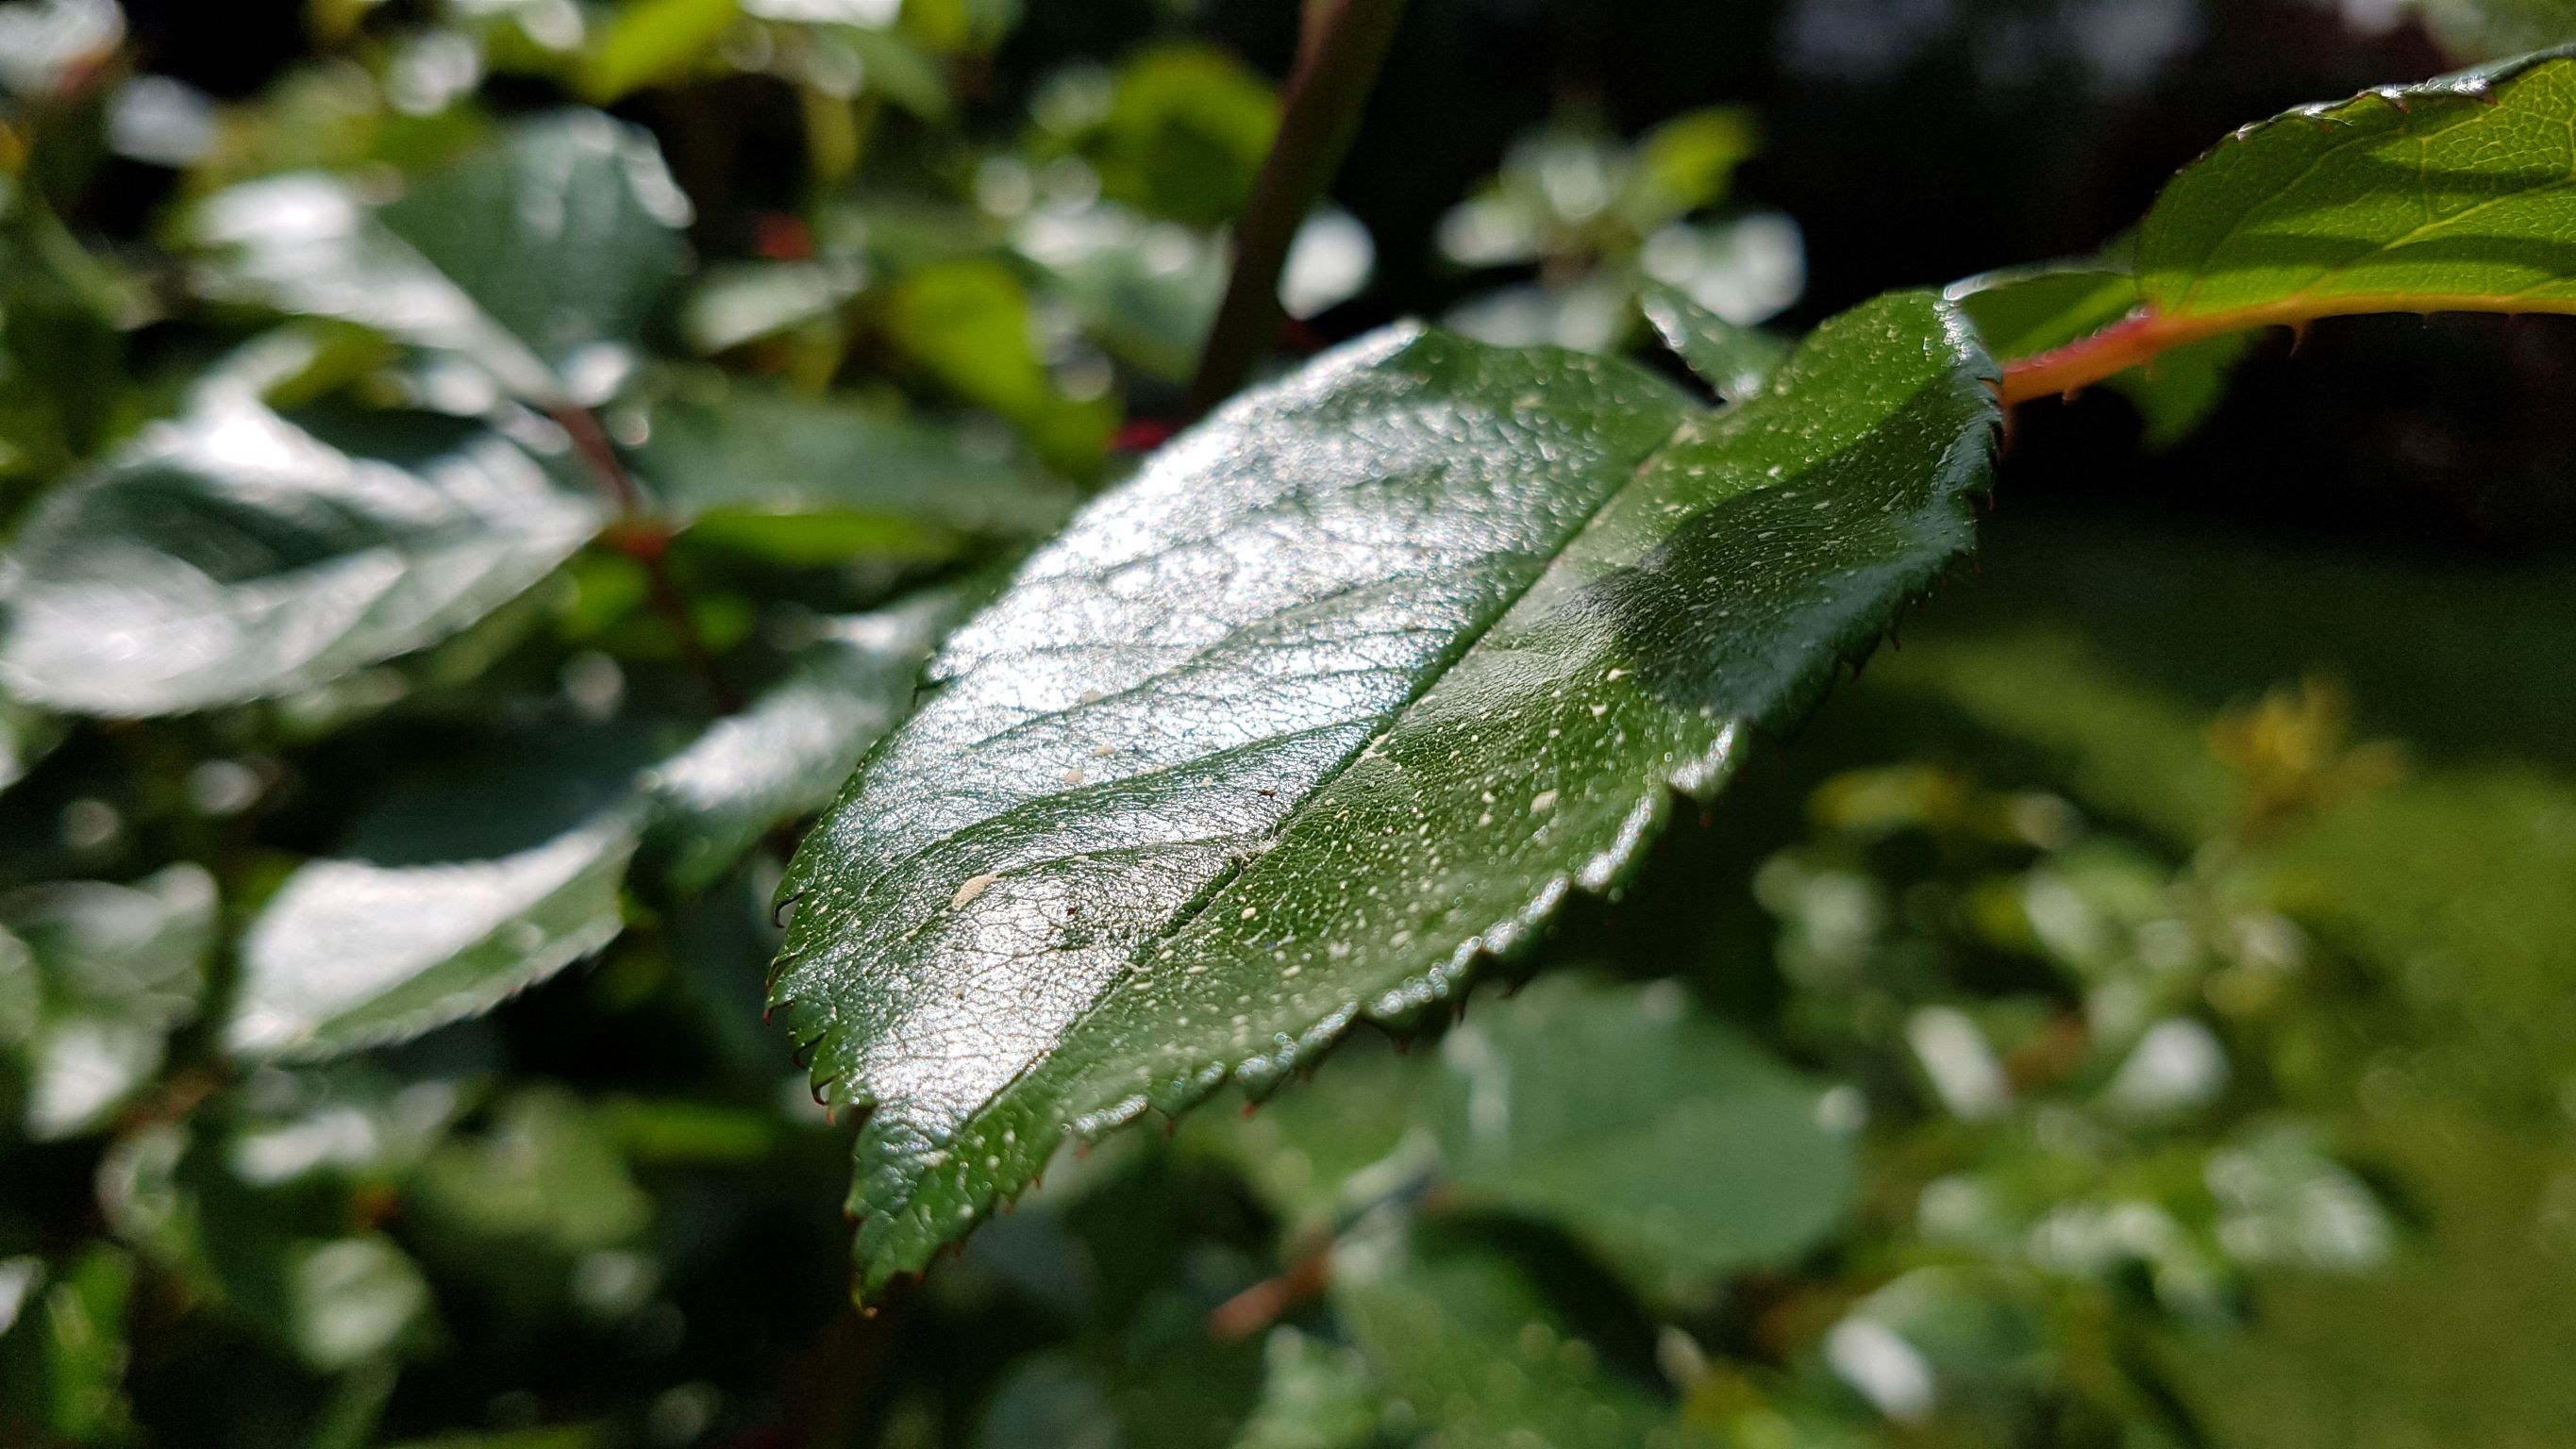
\includegraphics[width=0.5\linewidth]{img/leaf_gloss.jpg}
    % \includesvg[pretex=\tiny, width=1.0\linewidth]{img/pipeline}
    \caption[Leaf with glossy surface]{Real leafs often have a specular reflecting layer, therefore we incorporate a specular \ac{brdf} in our lighting calculations.}
    \label{fig:leaf_gloss}
\end{figure} 
The models we use neither have a specular map nor a specular color associated in their materials.
In order to still achieve the desired look it is possible to simply set the specular color to white, leading to a loss of structural information in the highlights.
Using the diffuse texture directly as a specular map results in colored highlights which does not match Figure \ref{fig:leaf_gloss}.
Therefore we first compute the luminosity of the diffuse texture which we then use as a specular map.
Figure \ref{fig:leaf_renderings} shows renderings of this approach.
\begin{figure}[ht]
    \centering
    \begin{subfigure}[b]{0.3\linewidth}
        \centering
        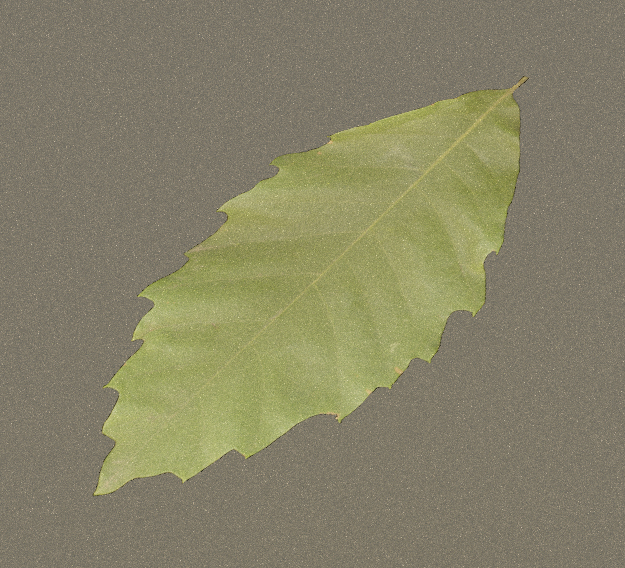
\includegraphics[width=1\linewidth]{img/leaf_no_spec.jpg}
        \caption{}
        % \label{fig:bounding_size_1}
    \end{subfigure}
    \begin{subfigure}[b]{0.3\linewidth}
        \centering
        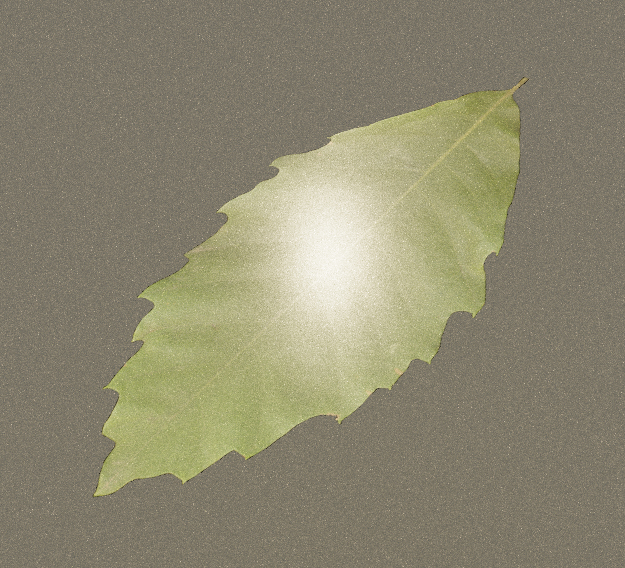
\includegraphics[width=1\linewidth]{img/leaf_spec.jpg}
        \caption{}
        % \label{fig:bounding_size_2}
    \end{subfigure}
	\caption[Comparison of renderings with and without specular maps]{Renderings of leafs using the default material (a) and our modification of converting the diffuse texture to a specular map (b).}
	\label{fig:leaf_renderings}
\end{figure}
We combine the diffuse and microfacet \ac{brdf} using the Fresnel term $F$ \cite{fresnel}, which describes the amount of light reflected on a surface.
It evaluates to values close to one for grazing angles and to one when light hits the surface perpendicularly \cite{pbr}.
For a layered surface the effect of the diffuse reflection is biggest near perpendicular angles while specular reflection mostly is visible near grazing angles \cite{pbr}.
We can therefore write our combined \ac{brdf} as:
\begin{equation*}
    f(\boldsymbol{x}, \omega_o, \omega_i) = F(|n_{\boldsymbol{x}} \cdot \omega_o|)f_{spec}(\boldsymbol{x}, \omega_o, \omega_i) + (1 - F(|n_{\boldsymbol{x}} \cdot \omega_o|))f_{diff}(\boldsymbol{x}, \omega_o, \omega_i).
\end{equation*}

As described in Section \ref{subsec:solving_beer_lambert_law_in_heterogeneous_media}, we use brick grid by \citeauthor{brick_grid} \cite{brick_grid} to represent the density values of a volume.
The authors also provide an implementation of the distance sampling procedure they use \cite{brick_grid}, which we rougly follow.
We use their distance sampling until we find an interaction and then perform a lookup in the NanoVDB grid to retrieve a filtered normal, diffuse and specular color, the index of refraction and the \ac{sggx} matrix $S$.
Since our procedure returns the albedo at this point of the medium, we now have to compute which frequencies of the light are absorbed, which is given by the color.
Just as for our surface rendering we apply the Fresnel term to weight the diffuse and specular color.
Because the Fresnel term requires a surface normal, we now use the filtered normal that we also stored in the NanoVDB grid.
We weight the specular color by $F$ and the diffuse color by $1-F$ to obtain our albedo.

At each sampled interaction in the medium we sample a new ray direction using the \ac{sggx} phase function.
Again we use the Fresnel term, this time to get a probability whether we should sample the diffuse phase function or the specular phase function.
Both phase functions rely on sampling a microflake normal from the \ac{sggx} \acl{vndf}.
% In contrast to \citeauthor{sggx} \cite{sggx}, we do not align this microflake normal with the ray direction $\omega_o$, but with the filtered normal $n$.
In contrast to \citeauthor{sggx} \cite{sggx}, we do not build a coordinate frame around the ray direction $\omega_o$, but we build it around the filtered normal $n$ to transform the microflake normal to world space.
Figure \ref{fig:tree_normal_maps} illustrates the normals of the mesh in world space and when the microflake normal is transformed with a coordinate frame around the direction $\omega_o$ or the filtered normal.
\begin{figure}[ht]
    \centering
    \begin{subfigure}[b]{0.3\linewidth}
        \centering
        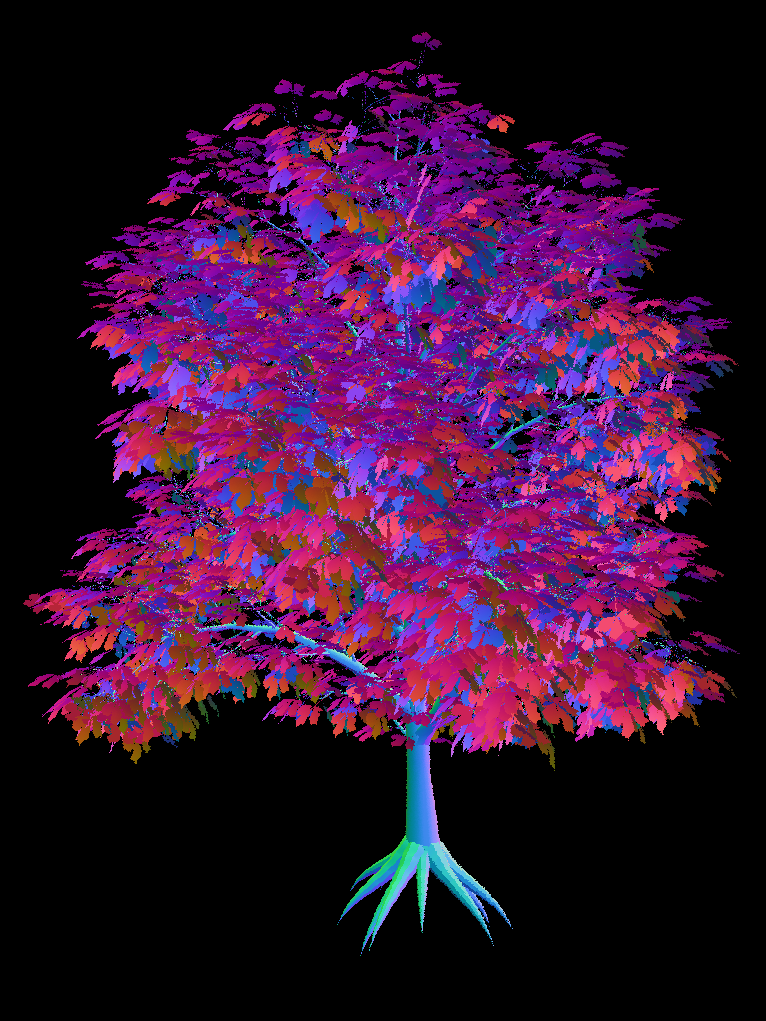
\includegraphics[width=1\linewidth]{img/normal_map_mesh.png}
        \caption{}
        % \label{fig:bounding_size_1}
    \end{subfigure}
    \begin{subfigure}[b]{0.3\linewidth}
        \centering
        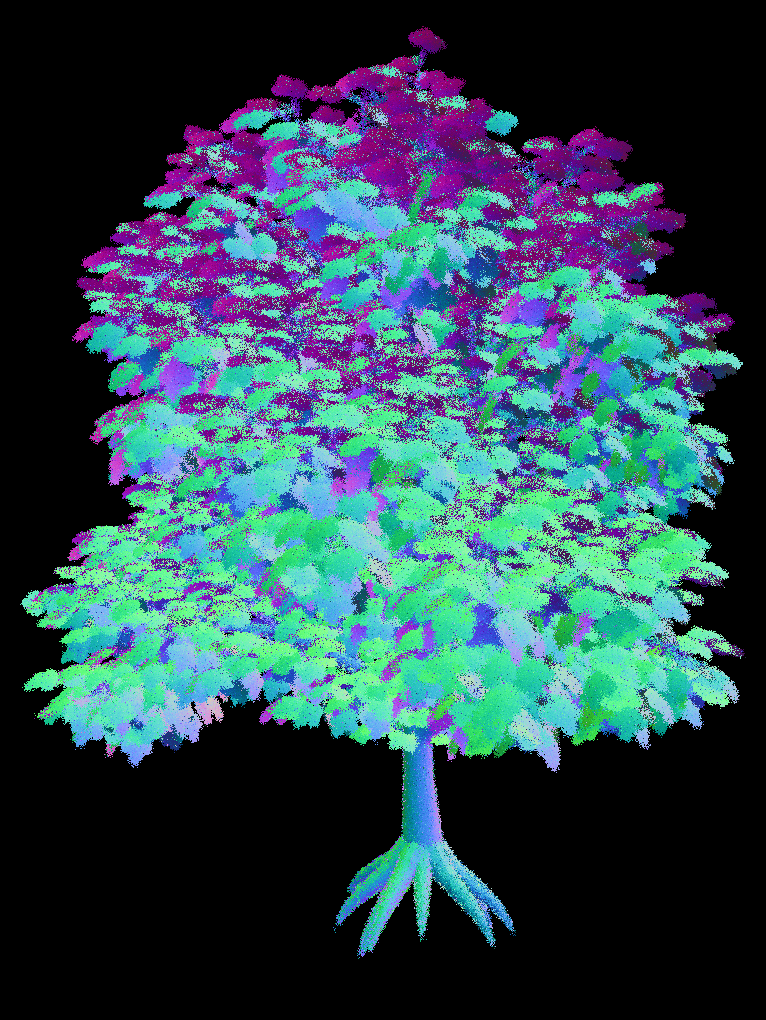
\includegraphics[width=1\linewidth]{img/normal_map_vndf_wo_aligned.png}
        \caption{}
        % \label{fig:bounding_size_2}
    \end{subfigure}
    \begin{subfigure}[b]{0.3\linewidth}
        \centering
        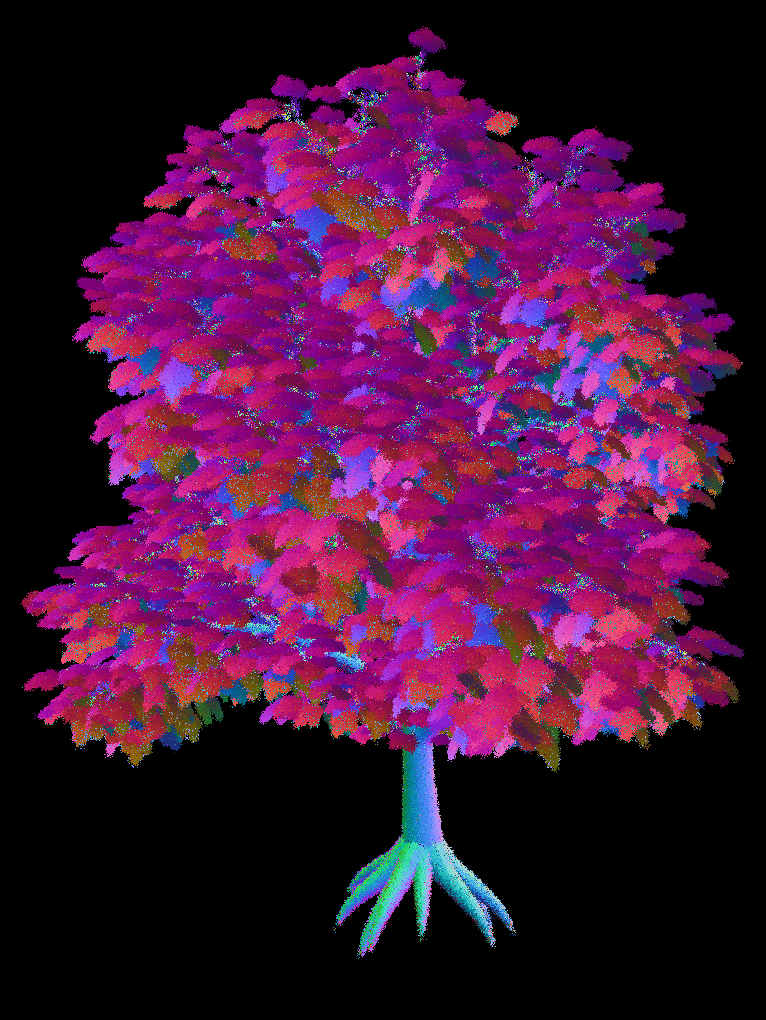
\includegraphics[width=1\linewidth]{img/normal_map_vndf_normal_aligned.png}
        \caption{}
        % \label{fig:bounding_size_1}
    \end{subfigure}
    \caption[Visualization of normals with meshes and volumes]{Visualization of the normals of the surface mesh (a), and of volumetric \acsp{lod} when the microflake normal is transformed with a coordinate frame around the direction $\omega_o$ (b) and when it is transformed with a coordinate frame around the filtered normal (c).
             Although being more blurry, transforming the microflake normal based on the filtered normal gives close results to the true normals.}
	\label{fig:tree_normal_maps}
\end{figure}
It is obvious, that transforming the microflake normal based on the outgoing direction $\omega_o$ gives different normals than the normals given by the mesh, while transforming it with a coordinate frame around the filtered normal gives normals that are distributed around the filtered normal.

Having sampled a reflection direction in the volume we move the origin of the new ray along this direction to the edge of the current voxel.
This is an idea by \citeauthor{vicini2021non} that prevents multiple scattering within a voxel \cite{vicini2021non}.
According to the authors multiple scattering can lead to paths passing through a voxel with a high density, which leads to an energy loss producing substantially darker looking volumes \cite{vicini2021non}.